\documentclass[12pt]{article}
\newif\ifshowsolutions
\showsolutionsfalse
%\showsolutionstrue

%% arXiv paper template by Flip Tanedo
%% last updated: Dec 2016



%%%%%%%%%%%%%%%%%%%%%%%%%%%%%
%%%  THE USUAL PACKAGES  %%%%
%%%%%%%%%%%%%%%%%%%%%%%%%%%%%

\usepackage{amsmath}
\usepackage{amssymb}
\usepackage{amsfonts}
\usepackage{graphicx}
\usepackage{xcolor}
\usepackage{nopageno}
\usepackage{enumerate}
\usepackage{parskip}
\usepackage{comment}
	
	
%http://tex.stackexchange.com/questions/15509/hide-custom-environment-content-based-on-boolean
\ifshowsolutions
	\newenvironment{solution}%
	{\color{blue!60!black}
	\textsf{\textbf{Solution}}:
	}%
	%
	{\ignorespacesafterend}
\else
	\excludecomment{solution}
\fi
	
%\newenvironment{solution}
%    {%\begin{sol}
%    \textcolor{blue!40!black}{
%	\textbf{Solution}:}
%    }
%    { 
%    %\end{sol}
%    }
%    
%%\includecomment{solution}




%%%%%%%%%%%%%%%%%%%%%%%%%%%%%%%%%
%%%  UNUSUAL PACKAGES        %%%%
%%%  Uncomment as necessary. %%%%
%%%%%%%%%%%%%%%%%%%%%%%%%%%%%%%%%

\usepackage{titlesec}
\titleformat*{\section}{\large\bfseries}

%% MATH AND PHYSICS SYMBOLS
%% ------------------------
%\usepackage{slashed}       % \slashed{k}
%\usepackage{mathrsfs}      % Weinberg-esque letters
%\usepackage{youngtab}	    % Young Tableaux
%\usepackage{pifont}        % check marks
\usepackage{bbm}           % \mathbbm{1} incomp. w/ XeLaTeX 
%\usepackage[normalem]{ulem} % for \sout


%% CONTENT FORMAT AND DESIGN (below for general formatting)
%% --------------------------------------------------------
\usepackage{lipsum}        % block of text (formatting test)
%\usepackage{color}         % \color{...}, colored text
%\usepackage{framed}        % boxed remarks
%\usepackage{subcaption}    % subfigures; subfig depreciated
%\usepackage{paralist}      % compactitem
%\usepackage{appendix}      % subappendices
%\usepackage{cite}          % group cites (conflict: collref)
%\usepackage{tocloft}       % Table of Contents	

%% TABLES IN LaTeX
%% ---------------
%\usepackage{booktabs}      % professional tables
%\usepackage{nicefrac}      % fractions in tables,
%\usepackage{multirow}      % multirow elements in a table
%\usepackage{arydshln} 	    % dashed lines in arrays

%% Other Packages and Notes
%% ------------------------
%\usepackage[font=small]{caption} % caption font is small



%\renewcommand{\thesection}{}
%\renewcommand{\thesubsection}{\arabic{subsection}}

%%%%%%%%%%%%%%%%%%%%%%%%%%%%%%%%%%%%%%%%%%%%%%%
%%%  PAGE FORMATTING and (RE)NEW COMMANDS  %%%%
%%%%%%%%%%%%%%%%%%%%%%%%%%%%%%%%%%%%%%%%%%%%%%%

\usepackage[margin=2cm]{geometry}   % reasonable margins

\graphicspath{{figures/}}	        % set directory for figures

% for capitalized things
\newcommand{\acro}[1]{\textsc{\MakeLowercase{#1}}}    

\numberwithin{equation}{section}    % set equation numbering
\renewcommand{\tilde}{\widetilde}   % tilde over characters
\renewcommand{\vec}[1]{\mathbf{#1}} % vectors are boldface

\newcommand{\dbar}{d\mkern-6mu\mathchar'26}    % for d/2pi
\newcommand{\ket}[1]{\left|#1\right\rangle}    % <#1|
\newcommand{\bra}[1]{\left\langle#1\right|}    % |#1>
\newcommand{\Xmark}{\text{\sffamily X}}        % cross out

% Change list spacing (instead of package paralist)
% from: http://en.wikibooks.org/wiki/LaTeX/List_Structures#Line_spacing
%\let\oldenumerate\enumerate
%\renewcommand{\enumerate}{
%  \oldenumerate
%  \setlength{\itemsep}{1pt}
%  \setlength{\parskip}{0pt}
%  \setlength{\parsep}{0pt}
%}

\let\olditemize\itemize
\renewcommand{\itemize}{
  \olditemize
  \setlength{\itemsep}{1pt}
  \setlength{\parskip}{0pt}
  \setlength{\parsep}{0pt}
}


% Commands for temporary comments
\newcommand{\flip}[1]{{\color{red} [\textbf{Flip}: {#1}]}}
\newcommand{\email}[1]{\texttt{\href{mailto:#1}{#1}}}

\newenvironment{institutions}[1][2em]{\begin{list}{}{\setlength\leftmargin{#1}\setlength\rightmargin{#1}}\item[]}{\end{list}}


\usepackage{fancyhdr}		% to put preprint number



% Commands for listings package
%\usepackage{listings}      % \begin{lstlisting}, for code
%
% \lstset{basicstyle=\ttfamily\footnotesize,breaklines=true}
%    sets style to small true-type


%%%%%%%%%%%%%%%%%%%%%%%%%%%%%%%%%%%%%%%%%%%%%%
%%%  TIKZ COMMANDS FOR EXTERNAL DIAGRAMS  %%%%
%%%  requires -shell-escape               %%%%
%%%  in texpad 1.7: prefs > shell esc sec %%%%
%%%%%%%%%%%%%%%%%%%%%%%%%%%%%%%%%%%%%%%%%%%%%%

%% This is for exporting tikz figures as into a ./tikz/ subfolder.
%% It is useful if you want pdf versions of the tikz diagrams or
%% if you need to speed up compilation of a large document with
%% many tikz diagrams.

%\write18{} % Careful with this!
%\usetikzlibrary{external}
%\tikzexternalize[prefix=tikz/] % folder for external pdfs


%%%%%%%%%%%%%%%%%%%
%%%  HYPERREF  %%%%
%%%%%%%%%%%%%%%%%%%

%% This package has to be at the end; can lead to conflicts
\usepackage{microtype}
\usepackage[
	colorlinks=true,
	citecolor=black,
	linkcolor=black,
	urlcolor=green!50!black,
	hypertexnames=false]{hyperref}



%%%%%%%%%%%%%%%%%%%%%
%%%  TITLE DATA  %%%%
%%%%%%%%%%%%%%%%%%%%%

%%% PREPRINT NUMBER USING fancyhdr
%%% Don't forget to set \thispagestyle{firststyle}
%%% ----------------------------------------------
%\renewcommand{\headrulewidth}{0pt} % no separator
%\fancypagestyle{firststyle}{
%\rhead{\footnotesize \texttt{UCI-TR-2016-XX}}}

\renewcommand{\thesubsection}{\thesection.\alph{subsection}}

\begin{document}

%\thispagestyle{empty}
%\thispagestyle{firststyle} %% to include preprint

\begin{center}

    {\Large \textsc{Homework 1:} 
    \textbf{Special Relativity}}


    
\end{center}

\vskip .4cm

\noindent
\begin{tabular*}{\textwidth}{rlcrll}
	\textsc{Course:}& Physics 208, {General Relativity} (Winter 2017)
	&
%	\hspace{1.2cm}
	&
	\\
	\textsc{Instructor:}& Flip Tanedo (\email{flip.tanedo@ucr.edu})
	&
	%\hfill
	&
	& 
	\\
	\textsc{Due Date:}& Tuesday, January 17 in class
	&
	%\hfill
	&
	%	
\end{tabular*}

You are required to complete the {\textsf{Reading Assignment}} and {\textsf{Essential Problems}} below. 
%
Please let me know if these are too time intensive\footnote{The `essential problems' are meant to be a bare minimum of independent work to follow the course.}.
%
You are invited to explore the `extra' problems as they apply to your goals for this course: {\textsf{Mathematical Problems}} develop geometric intuition, while {\textsf{Phenomenological Problems}} are applications of relativity. 
% 

\vspace{2em}
{\Large\textbf{\textsf{Reading Assignment}}}

Read the following topics in Hartle. You may choose to read the analogous topics in an appropriate textbook or reference of your preference.

\begin{itemize}
	\item Review chapters 1--3 as necessary depending on your background.
	\item Read chapters 4--5 on special relativity.
\end{itemize}


\vspace{2em}
{\Large\textbf{\textsf{Essential Problems}}}

\section{Pole-in-Barn (Hartle 4-3)}

A 20~m pole is carried so fast in the direction of its length that it appears to be only 10~m long in the lab frame. The funner carries the pole through the front door of a barn 10~m long. Just at the instant the head of the pole reaches the closed rear door, the front door can be closed, enclosing the pole within the 10~m barn for an instant. The rear door opens and the runner goes through. From the runner's point of view, however, the pole is 20~m long and the barn is only 5~m! Thus the pole can never be enclosed in the barn. Explain, quantitatively and by means of spacetime diagrams, the apparent paradox.


\begin{solution}
	Test
\end{solution}


\section{Black Hole Entropy and Dimensional Analysis}

When we were children, we used `unnatural units' with standard measures $L$ (e.g. $L$ = meter), $M$ (e.g. $M$ = kilogram), and $T$ (e.g. $T$ = second). For example, we say that the dimension of a velocity, $v$, is 
\begin{align}
	[v] = L/T \ .
\end{align}
As adults, we use natural units where $c = \hbar = 1$. What this really means is that we are free to use these quantities to convert between units---hence the term `lightyear' as a measure of distance. A `lightyear' is the distance that a photon travels in one year:
\begin{align}
	\text{light year} = c (1\text{ year})\ .
\end{align}

\subsection{The Planck Mass}

\begin{enumerate}[(i)]
\item Use the Newton force law, $F = G m_1m_2/r^2$, to determine the `unnatural' dimensions of the Newton constant, $G$. 
\item In natural units, we say that $G$ has \emph{mass dimension} $[G] = -2$, so that we can define a mass scale
\begin{align}
	M_P = \frac{1}{\sqrt{G}} \ .
\end{align}
This is called the \textbf{Planck mass}. Restore the factors of $\hbar$ and $c$ to make this definition correct in `unnatural' units. 
\end{enumerate}

\subsection{Hawking Radiation}

Black holes can evaporate by Hawking radiation\footnote{A cartoon picture of this process is as follows: quantum mechanics + special relativity tells us that the vacuum (`empty' space) is composed of virtual particle--anti-particle pairs. Near the event horizon of a black hole, one of these particles can fall into the black hole while the other radiates away as a physical particle.}. This means that black holes have a temperature. Use dimensional analysis to determine how this \textbf{Hawking temperature} scales with the mass of the black hole. 

\textsc{Hint}: there's one subtlety. There are two mass scales in the problem: the black hole mass, $M$, and the Planck mass, $M_P = 1/\sqrt{G}$. (In natural units, of course). In order to be able to use dimensional analysis, the additional piece of information is that $G$ is a gravitational coupling, so that gravitational effects should go like $GM$. 

How does $T_H$ scale with the combination $GM$? Observe that the black hole gets \emph{hotter} as it loses energy.

\subsection{The Holographic Principle}

Recall from thermodynamics that entropy, $S$, is related to energy $E$ and temperature $T$ by
\begin{align}
	\frac{dS}{dE} = \frac{1}{T} \ .
\end{align}
\begin{enumerate}[(i)]
	\item Identify the temperature with the Hawking temperature $T=T_H$ and set the energy to be the mass of the black hole so that $dE = dM$. Integrate with respect to the black hole mass to find how entropy scales with mass, $S \sim M^?$.
	\item The radius of the black hole's event horizon scales like $R = GM$. How does the black hole's entropy scale with its characteristic length scale? 
	\item Contrast the above result to the expected scaling of entropy in ordinary thermodynamics. Recall that entropy is an \emph{extensive} measure of the number of microstates in a system.
\end{enumerate}

The solution to this problem is spelled out in  the introduction to Zee's \emph{Einstein's Gravity in a Nutshell}. The `holographic principle' is the proposal that the properties of the black hole are encoded on its surface rather than its volume. This is analogous to how a hologram is a 3D image encoded onto a 2D surface. A manifestation of the holographic principle is the AdS/CFT correspondence, which posits that certain theories of strongly interacting systems in $d$-dimensions are mathematically identical to a weakly-coupled $(d+1)$-dimensional gravitational theory.




\vspace{2em}
{\Large\textbf{\textsf{Phenomenological Problems}}}

% From Cheng's Oxford GR book
This is a review of the `physical' derivation of the key results of special relativity from the single assumption that the speed of light is constant. As with all homework problems, you should do this if you haven't done it before or if the solution is not obvious to you.

\subsection{Time Dilation}

Imagine a light clock which marks off time by counting the number of times a photon bounces between two mirrored surfaces separated by a distance $L$ (Hartle Fig.~4.6). When the clock is in the same frame as you are, you observe that the time between `ticks' (a round trip between the mirrors) is $\Delta t = 2L/c$. What is the observed time between ticks if you measure the clock at it passes by you while relative to you with velocity $v$ perpendicular to the mirror axis? Confirm that it is $\Delta t' = \gamma \Delta t$. \textsc{Hint}: observe that now the photon travels with the same velocity but over a longer, diagonal path. 

\subsection{Length Contraction}

Here is a sketch of a Michelson--Morley experiment\footnote{If this is unfamiliar, try \url{http://lmgtfy.com/?q=michelson-morley+experiment}.} from Fig.~15-2 of \emph{The Feynman Lectures on Physics}, Volume I.	
%
% Feynman Lectures I, ch. 15
%\begin{figure*}[h!]
\begin{center}
	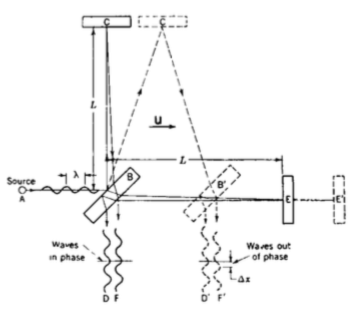
\includegraphics[width=.3\textwidth]{MMorleyFeynmanLecVolI.png}
	\end{center}
%\caption{Michelson--Morley experiment, figure 15-2 from \emph{The Feynman Lectures on Physics}, Volume I.	}
%\end{figure*}
%
Imagine a Michelson--Morley experiment set up on an imaginary, ideal train that is passing by you  with constant velocity $v$ as you sit at an imaginary train station. The two arms of the experiment have length $L$; one is aligned along the direction of the train and the other is perpendicular. There is no interference between the paths, so you conclude that the light waves must remain in phase.
\begin{enumerate}[(i)]
	\item Consider the arm $BE$ oriented along the direction of motion. What is the time, $t_1$ for a pulse of light to go from $B$ to $E$, accounting for the motion of the train with respect to you. Note that the mirror $E$ is moving away from the pulse.
	\item Do the same for the return trip, $t_2$, where now the mirror $B$ is moving towards the pulse.
	\item Do the same for the time $t_3$ for a pulse to traverse the diagonal path $BC$. Note that by symmetry, the return path takes the same time.
	\item Observe that $t_1 + t_2 \neq 2t_3$. However, if the length $L$ in parts (i) and (ii) is relabelled $L'$, then the results can be made equal if $L'$ is \emph{contracted} with respect to $L$. Show that this contraction is indeed $1/\gamma$.
\end{enumerate} 

%\vspace{2em}
%{\Large\textbf{\textsf{Advanced}}}
%
%\section{Weak Gravity Conjecture}

\vspace{2em}
{\Large\textbf{\textsf{Mathematical Problems}}}

\section{Electrodynamics}

\subsection{Maxwell Made Relativistic}

Classical electrodynamics obeys Lorentz invariance---Maxwell's equations know about special relativity. Indeed, Maxwell's equations can be formulated in a way that is manifestly relativistically invariant, writing everything in terms of the four-potential $A_\mu$, its field strength, $F_{\mu\nu} = \partial_\mu A_\nu - \partial_\nu A_\mu$, and the electromagnetic current $j_\mu$. Write this out explicitly, either using indices or differential forms\footnote{If you use differential forms, what type of $p$-form is the current?}. 

Observe that you can write this as two equations. One equation follows directly from the Bianchi identity, while the other comes from an action principle.

\subsection{Gauge redundancy}

The four-potential encodes the electromagnetic field. Indeed, quanta of $A_\mu$ are photons. Note that $A_\mu$ contains four degrees of freedom, whereas we know that the electromagnetic field only has two physical degrees of freedom: left- and right-polarizations (or linear combinations thereof). One degree of freedom is eliminated from the fact that the photon travels at the speed of light so that it can have no longitudinal polarization\footnote{A cartoon of this is to imagine a photon as a small ball. The photon cannot spin in the forward direction or else the top of the ball moves faster than $c$.}. The remaining degree of freedom is a degeneracy between our Lorentz-invariant mathematical description and the physical degrees of freedom. This degeneracy is called a gauge redundancy. Show that the physical electromagntic fields encoded in $F_{\mu\nu}$ are unchanged under $A_\mu(x) \to A_\mu(x) + \partial_\mu \alpha(x)$ for some gauge fixing function $\alpha(x)$. 

Observe that $\alpha(x)$ is an ``entire function's worth'' of arbitrariness---that is, at each point in spacetime, you can choose a different $\alpha$ (subject to smoothness).

Though we will not explore it in our course, the role of gauge theory is central in theoretical physics. In general relativity, you learn that the gravitational force can be understood as a curvature of spacetime, a differentiable manifold. In particle physics, one learns that the other fundamental forces of nature can be understood as \emph{gauge theories}. The connection between these pictures appears to run rather deep and continues to be an active research frontier under the banner of ``gravity is the square of gauge theory.''

%\section{Representation of the Lorentz Group} 
%
%The Lorentz transformations $\Lambda^{\mu}_{\phantom{\mu}\nu}$ form a group. As $4\times 4$ matrices, they act on 4-component vectors. For example, we recognize that for a given 4-momentum $p^\mu$ in some frame, one can transform into another frame which observes 4-momentum $p'^\mu = \Lambda^\mu_{\phantom\mu \nu} p^\nu$. However, there are other \textbf{representations} of the group, $D$. These are linear transformations that obey the group multiplication:
%\begin{align}
%	D(\Lambda_1) D(\Lambda_2) = D(\Lambda_1 \Lambda_2) \ ,
%\end{align}
%or in words:
%\begin{quote}
%	\emph{The `matrix' $D(\Lambda_1)$ corresponding to $\Lambda_1$ can be multiplied by the `matrix' $D(\Lambda_2)$ corresponding to $\Lambda_2$. The resulting `matrix' is the same as the matrix corresponding to $\Lambda_3 = \Lambda_1 \Lambda_2$.}
%\end{quote}
%These representations act linearly on a vector space with elements $\psi$. For example, a representation $D$ acting on tensors with two lower indices, $\psi = T_{\mu\nu}$ could be
%\begin{align}
%	D(\Lambda)_{\mu\nu}^{\phantom{\mu\nu}\rho\sigma} = \Lambda_\mu^{\phantom\mu\rho}\Lambda_\nu^{\phantom\nu\sigma} \ .
%\end{align}
%Ordinarily, one expects that similar re
%
%The solution to this problem is worked out in chapter~2.12 of Weinberg's \emph{Gravity and Cosmology} book. For a more thorough analysis that incorporates quantum physics, see chapter~2 of Wenberg's \emph{Quantum Theory of Fields}, Vol.~I.



\end{document}